\section{Présentation du projet}
\noindent La problématique à laquelle répond ce projet est présentée dans la Section \ref{sec:problematique}.
Une fois le sujet pris en main, nous nous sommes fixé des objectifs (Section \ref{sec:objectifs}) et avons mis en place une méthodologie (Section \ref{sec:methodologie}).

\subsection{Problématique}
\label{sec:problematique}
\noindent L’objectif de ce projet est de proposer des itinéraires cyclables sécurisés sur la zone géographique du sud bordelais, entre la place de la Victoire et le Campus universitaire de Talence/Pessac. 
Cet itinéraire est emprunté chaque jour par de nombreux étudiants, principalement en tramway via la ligne B.
Cependant, cette ligne est en saturation aux heures de pointe, et est régulièrement l’objet de pannes et d’incidents techniques.
Le vélo peut ainsi se dégager comme une bonne alternative.\\

\noindent La pratique du vélo est en expansion dans l'agglomération bordelaise.
Pendant l’année 2025, la pratique du vélo a augmenté de 6\% par rapport à 2024, en suivant la tendance des dernières années.
Cette hausse s'explique en partie par l'augmentation et l'amélioration des aménagements cyclables.\\

\noindent Le frein le plus important à la pratique du vélo est la problématique de la sécurité.
Le cycliste est un usager fragile et les accidents peuvent arrivés.
Il est donc important de séparer les usagers le plus possible pour éviter les sources d’incidents.\\

\subsection{Objectifs}
\label{sec:objectifs}
\noindent L’objectif de l’application est de proposer l’itinéraire qui convient le mieux en terme de compromis entre la sécurité et le temps de trajet, en s’adaptant au profil de l’utilisateur.\\

\noindent Pour proposer une expérience personnalisée, le calcul d'itinéraires prend en compte le type de vélo qu'utilise le client, son endurance ainsi que ses préférences.
Ainsi, l'application propose des trajets qui peuvent convenir à chacun, pour permettre à tous une pratique sécurisée du vélo.\\

\noindent Pour toucher un maximum d'utilisateurs, le projet consiste au développement d'une application Web mais aussi d'une application mobile.
Sur chacune d'elles, l'utilisateur peut créer son compte, afin de stocker ses informations.
Il a donc un accès facilité à ses adresses de préférence, notamment celle de son domicile et de son lieu de travail, pour une utilisation quotidienne rapide et efficace.\\

\subsection{Méthodologie}
\label{sec:methodologie}
\noindent Pour mener à bien ce projet, nous avons suivi des méthodes de Génie Logiciel.
Nous avons commencé par établir, en accord avec les clients, un cahier des charges \cite{CahierDesCharges}.
Celui-ci décrit les différents objectifs fixé au début du projet, et contient un diagramme de Gant (Figure \ref{fig:gant}) pour organiser les différentes tâches à effectuer.

\begin{figure}[H]
    \centering
    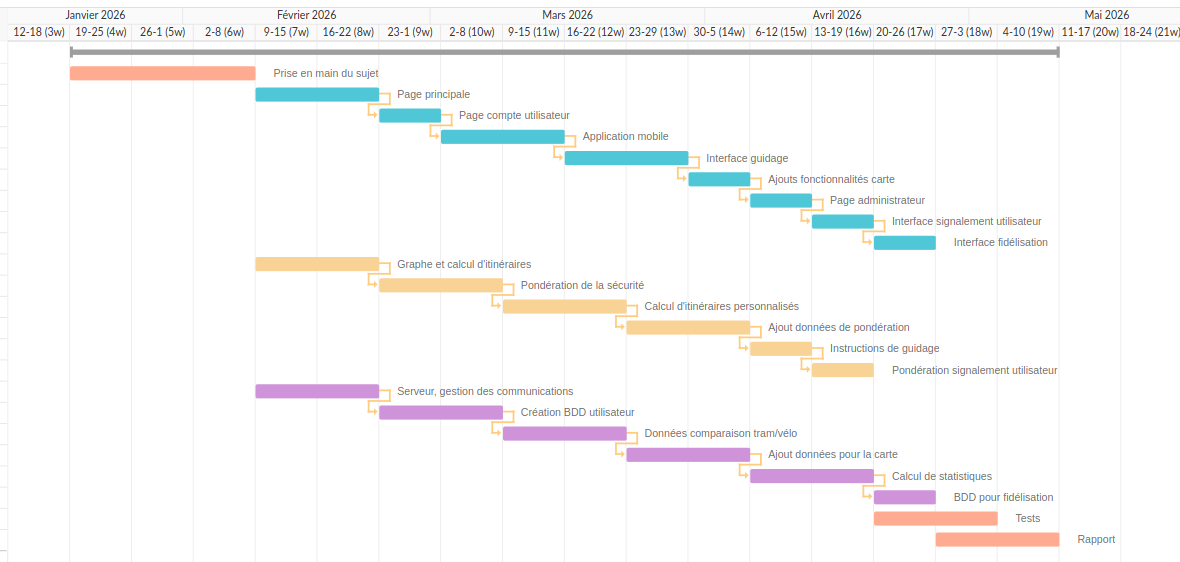
\includegraphics[width=\textwidth]{img/gant.png}
    \caption{Diagramme de Gant du projet.}
    \label{fig:gant}
\end{figure}

\noindent Le développement du projet s'est déroulé sur 16 semaines, du 19 janvier au 7 mai.\\

\noindent Comme montré sur le diagramme de Gant, nous nous sommes répartis en trois équipes.

\noindent Une première équipe composée de Joan Dumarchat et Léia Daragnès a pris en charge le calcul des itinéraires sécurisés.
Comme expliqué dans la Section \ref{sec:graphes}, le travail consistait à générer des graphes correspondant aux routes et à calculer des itinéraires sécurisés en prenant en compte différents paramètres.

\noindent Une seconde équipe composée de Khaoula Najmeddine et Angelo Tunney s'est concentrée sur l'API.
Ils ont donc mis en place chaque requête et ont construit la base de données nécessaire au projet, comme décrit dans la Section \ref{sec:backend}.

\noindent Une troisième et dernière équipe composée de Alexis Gaudray Bouju et Matheline Chevalier s'est occupée du développement Frontend.
Ils ont développé dans un premier temps le site Web, puis l'application mobile, en utilisant les technologies décrites dans la Section \ref{sec:frontend}.\\

\noindent Pour avoir un suivi régulier de notre travail, nous avons organisé toutes les une ou deux semaines une réunion avec nos encadrants.
À chaque réunion, nous exposions le travail effectué et les divers problèmes rencontrés.

\noindent De plus, pour pouvoir suivre l'avancement de chaque équipe, nous avons créé une fiche de suivi du projet.
Sur celle-ci se trouve le détail de chaque tâche à effectuer, ainsi que l'avancement de chaque équipe.\\

\noindent Pour permettre un développement et une mise en commun du code efficace, nous avons dans un premier temps créé un dépôt Git sur la Forge fournie par l'Enseirb Matmeca.
Pour pouvoir partager notre code à l'ensemble des encadrants, nous avons ensuite créé un dépôt GitHub open source \cite{GitHub}.